\documentclass[11pt,a4paper]{article}
\usepackage[a4paper,top=2.4cm,bottom=2.4cm,left=2.7cm,right=2.7cm]{geometry}
\usepackage[T5]{fontenc}
\usepackage[utf8]{inputenc}
\usepackage[vietnamese]{babel}
\usepackage{lmodern}
\usepackage{amsmath,amssymb,booktabs,array,graphicx,microtype,siunitx}
\usepackage{setspace,titlesec,fancyhdr,float}
\usepackage[hidelinks]{hyperref}
\graphicspath{{reports/figures/}{figures/}}
\sisetup{output-decimal-marker={,}}
\setstretch{1.15}
\setlength{\parindent}{0pt}
\setlength{\parskip}{6pt plus 1pt minus 1pt}
\renewcommand{\arraystretch}{1.16}
\titleformat{\section}{\large\bfseries}{\thesection.}{0.6em}{}
\titleformat{\subsection}{\normalsize\bfseries}{\thesubsection.}{0.6em}{}
\pagestyle{fancy}
\fancyhf{}
\fancyhead[L]{\small Uncertainty-aware DINOv3 Retrieval}
\fancyhead[R]{\small E1 và E2B}
\fancyfoot[C]{\thepage}
\renewcommand{\headrulewidth}{0.4pt}
\renewcommand{\abstractname}{Tóm tắt}

\title{\bfseries\LARGE So sánh độ bất định theo ảnh và độ tin cậy theo cặp\\[0.3em]
trong truy hồi ảnh với DINOv3}
\author{Báo cáo tổng hợp thực nghiệm E1 và E2B}
\date{17 tháng 9 năm 2026}

\begin{document}
\maketitle
\thispagestyle{plain}

\begin{abstract}
Báo cáo tổng hợp hai hướng sử dụng độ tin cậy cho truy hồi ảnh trên
CUB-200-2011. E1 gán một uncertainty score cho từng ảnh và dùng score này để
sắp lại Top-$N$. E2B học Pair-wise Confidence trực tiếp cho từng cặp ảnh truy
vấn--ứng viên, sau đó đánh giá riêng confidence và phép kết hợp với cosine.
Mọi so sánh E2B dùng cùng frozen DINOv3 CLS embedding, cùng danh sách ứng viên
và $N\in\{10,20,50,100\}$.

Kết quả cho thấy Image Uncertainty không phù hợp để thay thế thứ tự cosine:
ở E1, Recall@1 giảm từ \SI{87.9980}{\percent} xuống
$\SI{79.8447}{\percent}\pm\SI{0.2108}{\percent}$ tại $N=10$ và còn
\SI{27.2676}{\percent} tại $N=100$. Trong phép so sánh E2B dùng cùng tập train,
Pair-wise Confidence luôn tốt hơn Image Uncertainty nhưng vẫn thấp hơn
baseline. Fusion với $\lambda=0{,}75$ giữ nguyên Recall@1
\SI{88.0149}{\percent}, đồng thời tăng nhẹ Recall@2/4/8. Các khoảng bootstrap
95\% đều chứa 0, vì vậy chưa có bằng chứng rằng Fusion cải thiện Recall@1.

\textbf{Từ khóa:} DINOv3, truy hồi ảnh, uncertainty, pair-wise confidence,
reranking.
\end{abstract}

\section{Mục tiêu}
Hai thực nghiệm trả lời hai câu hỏi liên tiếp:
\begin{enumerate}
  \item Uncertainty của một ảnh có thể dùng để sắp lại kết quả cosine hay không?
  \item Nếu không, confidence học trực tiếp trên một cặp ảnh có giữ lại thông
  tin phù hợp hơn cho truy hồi hay không?
\end{enumerate}

E1 và E2B đều giữ nguyên backbone DINOv3. E1 chạy ba seed để đo mức biến động
của EDL head. E2B là một lần chạy seed 42; kết quả E2B vì vậy được báo cáo là
single-seed result, không trình bày mean $\pm$ std.

\section{Phương pháp}
\subsection{DINOv3 Baseline}
Với ảnh $x$, final CLS token được chuẩn hóa L2:
\begin{equation}
 z(x)=\frac{h_{\mathrm{cls}}(x)}{\lVert h_{\mathrm{cls}}(x)\rVert_2},
 \qquad s_{\cos}(q,x)=z(q)^\top z(x).
\end{equation}
Gallery được xếp theo cosine giảm dần và loại chính ảnh truy vấn. Đây là R0
trong E1 và DINOv3 Baseline trong E2B.

\subsection{Image Uncertainty}
EDL head nhận CLS feature 768 chiều và sinh evidence, $\alpha$ và uncertainty:
\begin{equation}
 e_k=\operatorname{softplus}(f_k(x)),\qquad
 \alpha_k=e_k+1,\qquad
 u(x)=\frac{K}{\sum_{k=1}^{K}\alpha_k},\quad K=100.
\end{equation}
Image Uncertainty Reranking giữ nguyên tập ứng viên cosine, chỉ sắp lại $N$ ảnh
đầu theo $u(x)$ tăng dần. Các ảnh ngoài Top-$N$ không được đưa lên trên.

\subsection{Evidential Embedding}
Nhánh này dùng trực tiếp vector $\boldsymbol\alpha$ và khoảng cách L2:
\begin{equation}
 d_{\alpha}(q,x)=\lVert\boldsymbol\alpha(q)-\boldsymbol\alpha(x)\rVert_2.
\end{equation}
Cách biểu diễn này dựa trên Evidential Transformers, nhưng backbone được thay
bằng DINOv3 nên được xem là một adaptation, không phải tái lập nguyên bản.

\subsection{Pair-wise Confidence và Fusion}
Mạng MLP nhận hai embedding theo thứ tự cố định query trước, candidate sau:
\begin{align}
 \phi(q,x)&=[z(q);z(x);|z(q)-z(x)|],\\
 C(q,x)&=\sigma\!\left(\operatorname{MLP}(\phi(q,x))\right).
\end{align}
MLP có kiến trúc $2304\rightarrow512\rightarrow128\rightarrow1$, ReLU và
dropout 0,1. Mạng được train bằng Binary Cross Entropy trên số positive và
negative pairs bằng nhau. Negative gần nhất được lấy một lần từ cosine
Top-100 trên fit set và không cập nhật online.

Fusion dùng điểm
\begin{equation}
 S_{\lambda}(q,x)=\lambda s_{\cos}(q,x)+(1-\lambda)C(q,x).
\end{equation}
Các giá trị $\lambda\in\{0;0{,}25;0{,}5;0{,}75;0{,}9;1\}$ đều được lưu.
$\lambda=0$ là Pair-wise Confidence, còn $\lambda=1$ tái tạo baseline.

\section{Thiết lập thực nghiệm}
CUB-200-2011 gồm 11.788 ảnh. Classes 0--99 tạo tập development 5.864 ảnh;
classes 100--199 tạo tập test 5.924 ảnh chưa xuất hiện khi train. Development
được chia theo từng lớp thành 4.687 ảnh fit và 1.177 ảnh validation với seed
chia dữ liệu cố định bằng 42.

Backbone là \texttt{facebook/dinov3-vitb16-pretrain-lvd1689m}, revision
\texttt{5931719e67bbdb9737e363e781fb0c67687896bc}, ảnh đầu vào
$224\times224$. Thực nghiệm chạy bằng Python 3.12.13, PyTorch 2.10.0,
CUDA 12.8 và hai Tesla T4. Metrics là Recall@1/2/4/8.

Trong E1, ba seed 42, 43 và 44 dùng cùng fit/validation split. Sau khi chọn
epoch và $N$ trên validation, EDL head được train lại trên toàn development để
đánh giá test. Trong phép so sánh E2B, EDL control và Pair-wise Confidence đều
chỉ train trên 4.687 ảnh fit. Checkpoint Pair-wise Confidence được chọn theo
validation BCE tại epoch 19. $\lambda=0{,}75$ được chọn trên hàng $N=100$ của
validation theo Hits@1 $\rightarrow$ Hits@2 $\rightarrow$ Hits@4
$\rightarrow$ Hits@8 $\rightarrow$ $\lambda$ lớn hơn.

\section{Kết quả E1: uncertainty theo ảnh}
\subsection{Kết quả chính}
\begin{table}[H]
\centering
\caption{Recall@K trên test, mean $\pm$ sample standard deviation qua ba seed
(\%). R1 dùng $N=10$ được chọn trên validation.}
\begin{tabular}{@{}lrrrr@{}}
\toprule
Phương pháp & R@1 & R@2 & R@4 & R@8\\ \midrule
R0: DINOv3 cosine & 87,9980 & 92,7583 & 95,2566 & 97,0122\\
R1: Image Uncertainty
& $79,8447\pm0,2108$ & $88,3075\pm0,2000$
& $93,9849\pm0,0639$ & $96,8490\pm0,0195$\\
\bottomrule
\end{tabular}
\end{table}

R1 giảm trung bình 8,1533 điểm phần trăm tại R@1. Paired bootstrap 95\% của
R@1 hoàn toàn dưới 0 ở cả ba seed: $[-8{,}9129;-6{,}9379]$,
$[-9{,}1661;-7{,}2586]$ và $[-9{,}3180;-7{,}3430]$ điểm phần trăm. Kết quả
không hỗ trợ giả thuyết rằng uncertainty theo ảnh cải thiện thứ hạng cosine.

\subsection{Ảnh hưởng của Top-$N$}
\begin{table}[H]
\centering
\caption{Image Uncertainty theo Top-$N$ trên test, trung bình ba seed (\%).}
\begin{tabular}{@{}crrrr@{}}
\toprule
$N$ & R@1 & R@2 & R@4 & R@8\\ \midrule
10  & 79,8447 & 88,3075 & 93,9849 & 96,8490\\
20  & 72,5073 & 83,1702 & 91,2953 & 96,0556\\
50  & 51,1591 & 64,3991 & 78,8375 & 90,3050\\
100 & 27,2676 & 38,7857 & 53,8431 & 70,6842\\
\bottomrule
\end{tabular}
\end{table}

Khi $N$ tăng, nhiều ảnh vốn được cosine đặt đúng bị đưa xuống dưới. Vì vậy
$N=10$ là lựa chọn ít bất lợi nhất, không phải một cấu hình vượt baseline.

\section{Kết quả E2B: confidence theo cặp}
\subsection{So sánh năm phương pháp}
\begin{table}[H]
\centering
\caption{Kết quả trên 5.924 test queries (\%). Ba phương pháp reranking dùng
cùng $N=100$; EDL control và Pair-wise Confidence cùng train trên fit set.}
\begin{tabular}{@{}lrrrr@{}}
\toprule
Phương pháp & R@1 & R@2 & R@4 & R@8\\ \midrule
DINOv3 Baseline & \textbf{88,0149} & 92,7583 & 95,2566 & 97,0122\\
Evidential Embedding & 34,4868 & 44,9021 & 55,6550 & 66,4078\\
Image Uncertainty & 27,3801 & 41,3403 & 57,1911 & 73,8521\\
Pair-wise Confidence & 78,9163 & 88,6563 & 93,8049 & 96,5057\\
Fusion ($\lambda=0{,}75$) & \textbf{88,0149} & \textbf{92,7920}
& \textbf{95,3410} & \textbf{97,0459}\\
\bottomrule
\end{tabular}
\end{table}

Fusion giữ nguyên 5.214 Hits@1 như baseline. R@2 tăng 2 query, R@4 tăng 5
query và R@8 tăng 2 query. Paired bootstrap 95\% của chênh lệch Fusion--baseline
lần lượt là $[-0{,}3038;0{,}3376]$, $[-0{,}2363;0{,}3038]$,
$[-0{,}1350;0{,}2870]$ và $[-0{,}1519;0{,}2194]$ điểm phần trăm. Tất cả đều
chứa 0, do đó các thay đổi nhỏ này chưa đủ để kết luận có cải thiện ổn định.

\subsection{So sánh công bằng theo Top-$N$}
\begin{table}[H]
\centering
\caption{Recall@1 theo cùng số ứng viên được sắp lại (\%). Fusion dùng
$\lambda=0{,}75$ đã chọn trên validation.}
\begin{tabular}{@{}crrr@{}}
\toprule
$N$ & Image Uncertainty & Pair-wise Confidence & Fusion\\ \midrule
10  & 80,3174 & 84,7907 & 88,0149\\
20  & 73,5989 & 83,7779 & 88,0149\\
50  & 53,9669 & 81,2289 & 88,0149\\
100 & 27,3801 & 78,9163 & 88,0149\\
\bottomrule
\end{tabular}
\end{table}

Pair-wise Confidence tốt hơn Image Uncertainty ở mọi $N$. Tuy nhiên, khi dùng
đơn lẻ, cả hai đều thấp hơn cosine baseline. Điều này cho thấy quan hệ giữa
query và candidate phù hợp với retrieval hơn uncertainty của candidate riêng
lẻ, nhưng confidence vẫn chưa đủ chính xác để thay hoàn toàn cosine.

\begin{figure}[H]
\centering
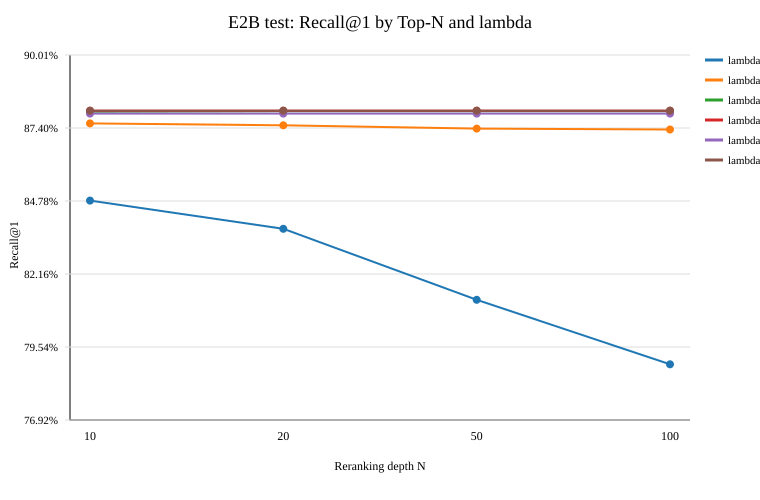
\includegraphics[width=0.88\textwidth]{e2b_topn_lambda_recall1.png}
\caption{Recall@1 của Fusion theo Top-$N$ và $\lambda$. $\lambda=0{,}75$ giữ
R@1 ngang baseline ở cả bốn $N$; các $\lambda$ nhỏ làm confidence chi phối và
giảm kết quả khi $N$ tăng.}
\label{fig:lambda-grid}
\end{figure}

\subsection{Ảnh hưởng của $\lambda$ tại $N=100$}
\begin{table}[H]
\centering
\caption{Fusion grid trên test tại $N=100$ (\%).}
\begin{tabular}{@{}crrrr@{}}
\toprule
$\lambda$ & R@1 & R@2 & R@4 & R@8\\ \midrule
0    & 78,9163 & 88,6563 & 93,8049 & 96,5057\\
0,25 & 87,3396 & 92,2687 & 95,3579 & 97,0966\\
0,50 & 87,9980 & 92,5219 & \textbf{95,4254} & 97,0966\\
0,75 & \textbf{88,0149} & \textbf{92,7920} & 95,3410 & 97,0459\\
0,90 & 87,9136 & 92,7076 & 95,3410 & 97,0797\\
1    & \textbf{88,0149} & 92,7583 & 95,2566 & 97,0122\\
\bottomrule
\end{tabular}
\end{table}

Kết quả tốt nhất không xuất hiện khi confidence đứng một mình. Confidence chỉ
hữu ích như một tín hiệu phụ có trọng số nhỏ bên cạnh cosine.

\section{Phân tích độ tin cậy và failure cases}
Trên toàn bộ 592.400 cặp ứng viên test, Pair-wise Confidence đạt AUROC 0,7054,
AUPRC 0,6365, Brier score 0,3646 và ECE 0,3689. Ở candidate cosine Top-1,
AUROC là 0,6287 và ECE là 0,0833. Confidence có khả năng phân biệt nhất định
nhưng chưa được hiệu chỉnh tốt trên toàn bộ Top-100; phần lớn score tập trung
ở khoảng 0,9--1,0.

\begin{figure}[H]
\centering
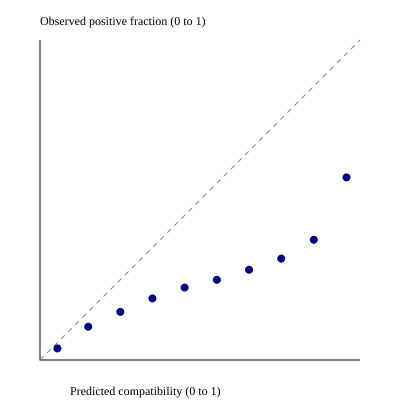
\includegraphics[width=0.55\textwidth]{e2b_candidate_calibration.png}
\caption{Biểu đồ calibration của Pair-wise Confidence trên các cặp ứng viên
test. Đường đứt thể hiện trường hợp score khớp hoàn toàn tỉ lệ cặp cùng lớp.}
\end{figure}

Tại $N=100$, Image Uncertainty sửa đúng 134 query nhưng làm sai thêm 3.726
query. Pair-wise Confidence sửa đúng 213 và làm sai 752 query. Fusion cân bằng
đúng 47 query được sửa và 47 query bị làm sai, nên tổng Hits@1 không đổi.

\begin{figure}[H]
\centering
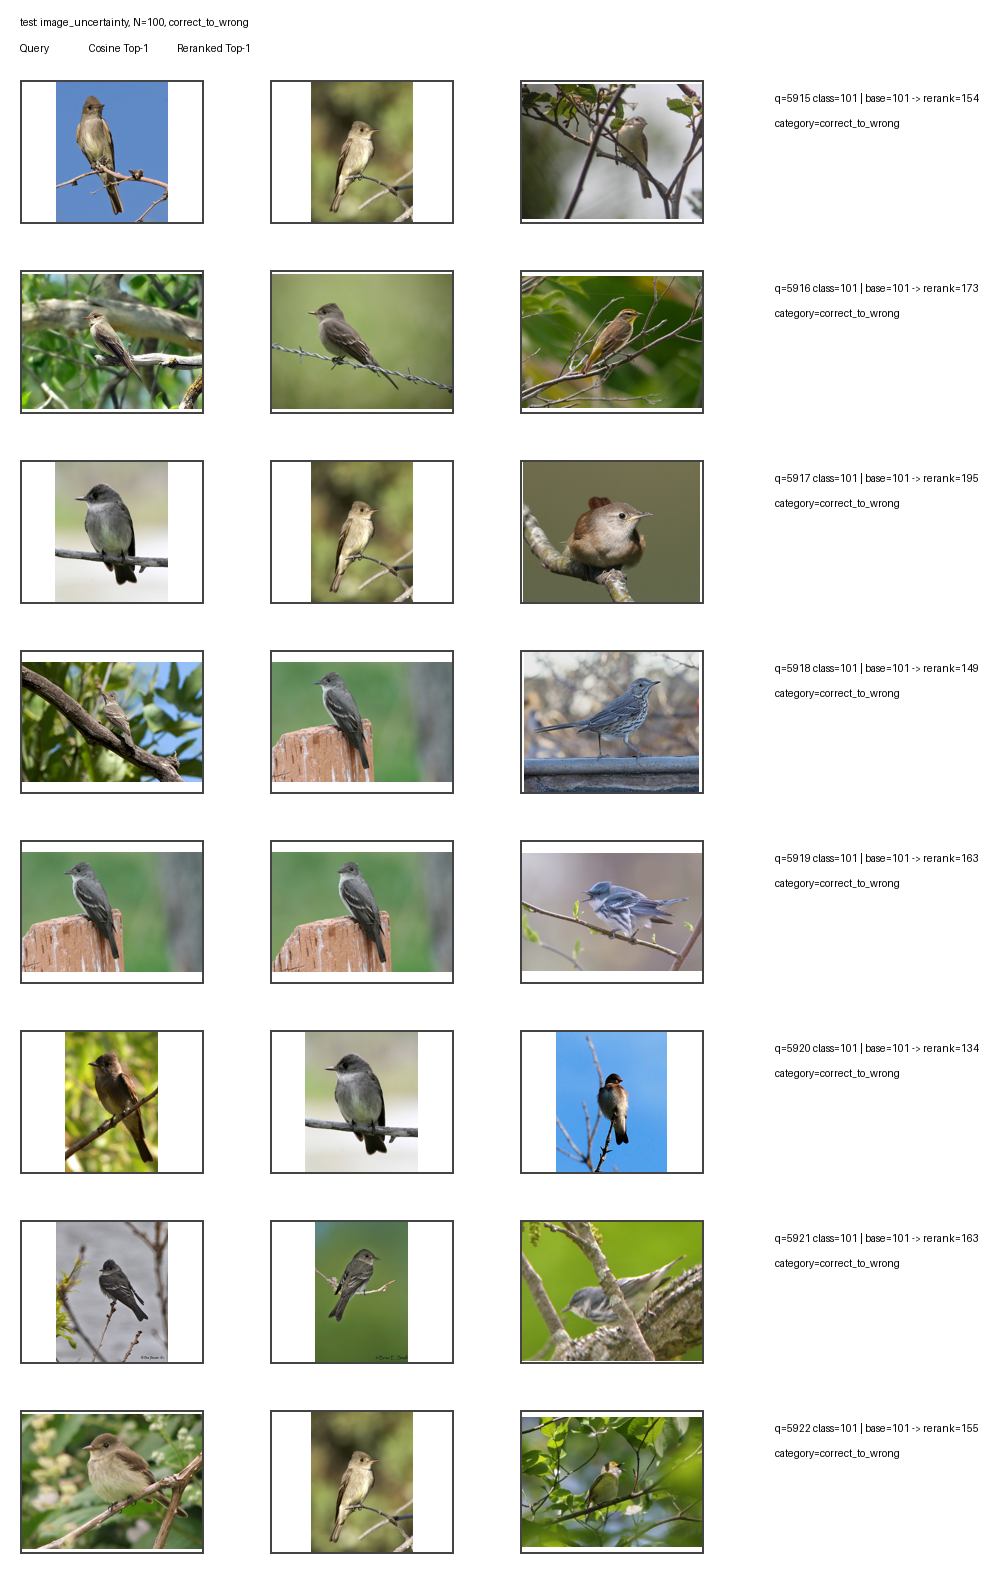
\includegraphics[width=0.92\textwidth]{image_uncertainty_correct_to_wrong.png}
\caption{Các trường hợp Image Uncertainty $N=100$ làm kết quả cosine đúng
thành sai. Cột trái là query, giữa là cosine Top-1, phải là kết quả sau rerank.}
\end{figure}

\begin{figure}[H]
\centering
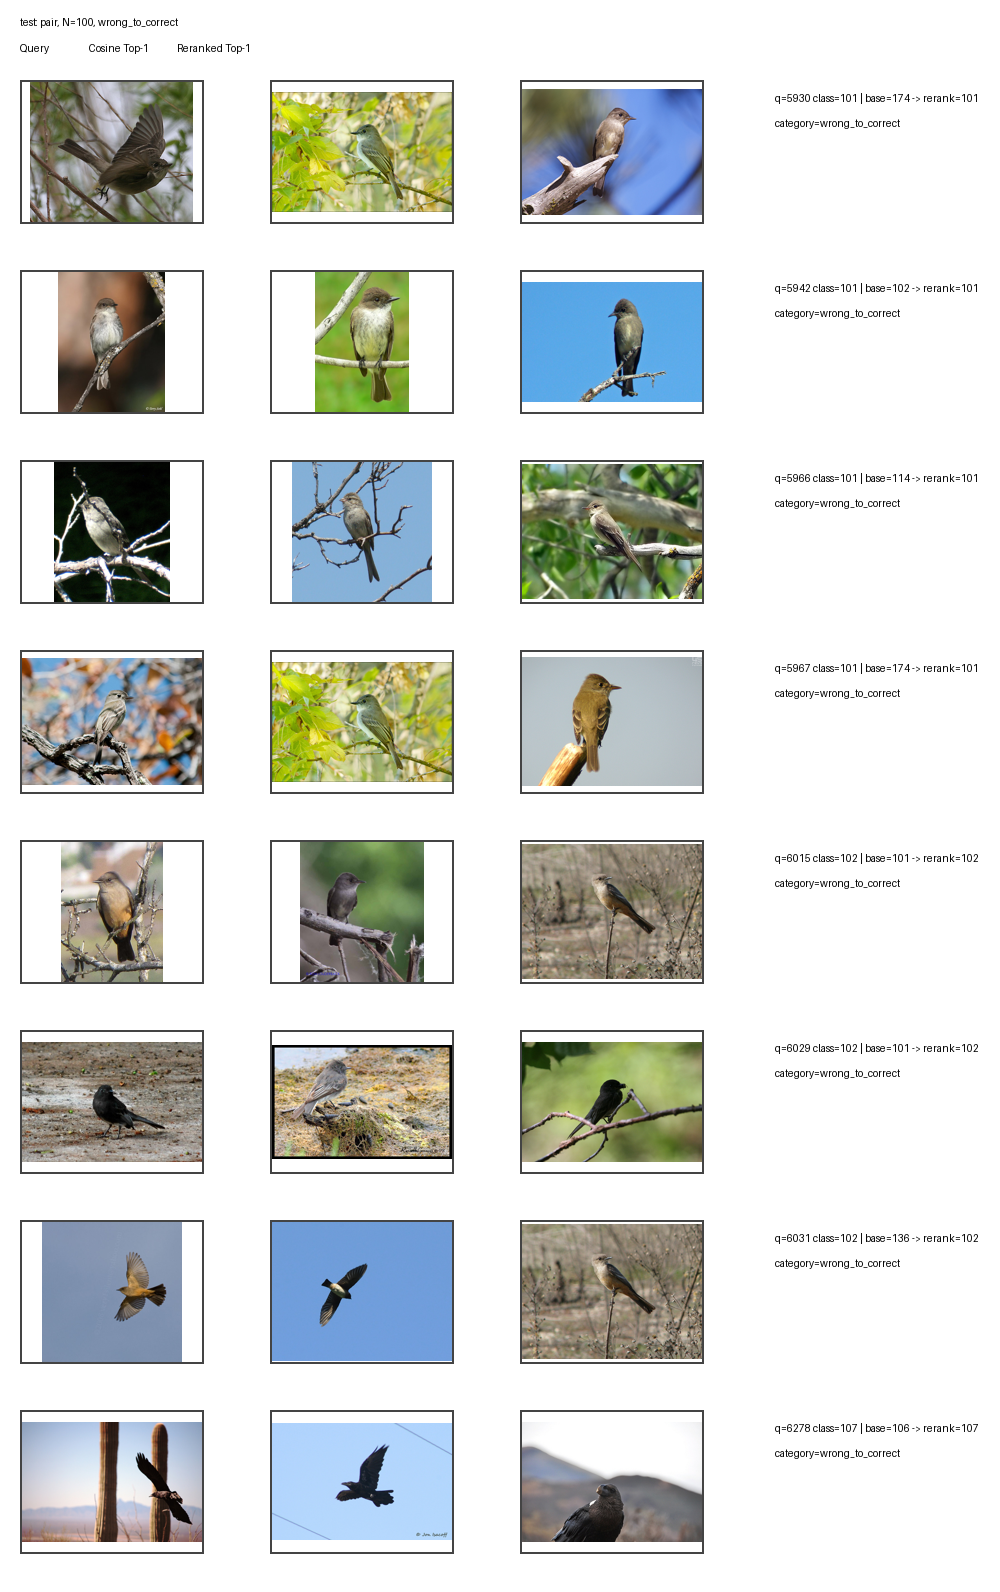
\includegraphics[width=0.92\textwidth]{pair_wrong_to_correct.png}
\caption{Các trường hợp Pair-wise Confidence $N=100$ sửa kết quả cosine sai
thành đúng. Mô hình thường đưa lên ảnh có hình dáng và chi tiết loài gần query.}
\end{figure}

\begin{figure}[H]
\centering
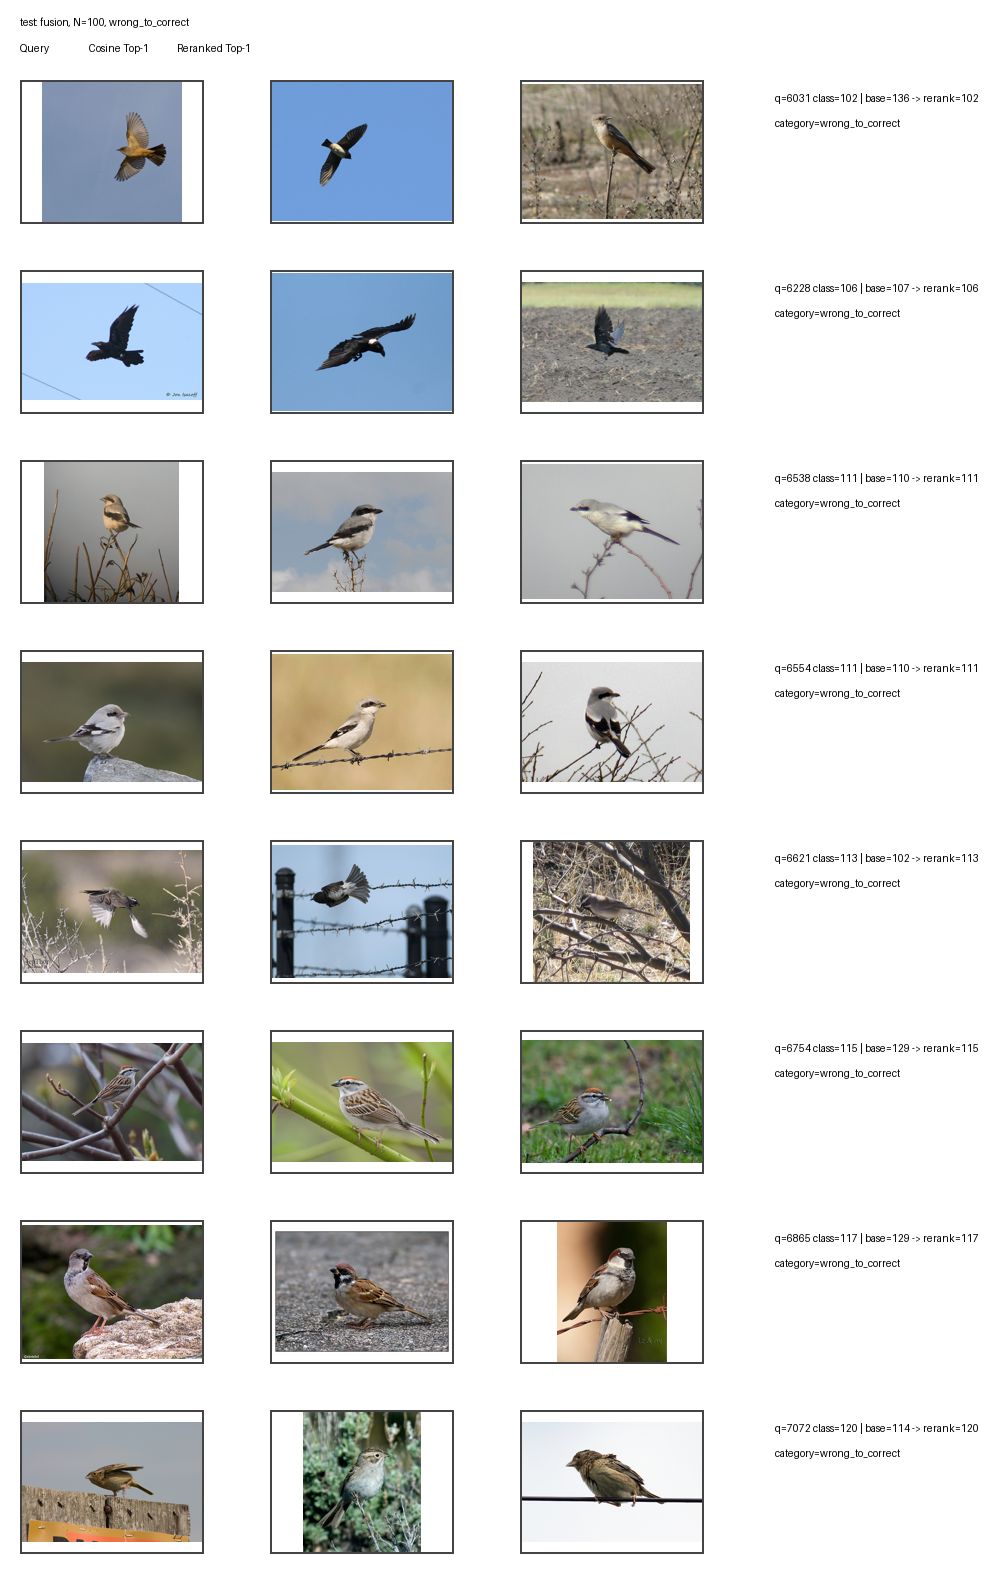
\includegraphics[width=0.92\textwidth]{fusion_wrong_to_correct.png}
\caption{Các trường hợp Fusion $N=100$, $\lambda=0{,}75$ sửa đúng Top-1.}
\end{figure}

\begin{figure}[H]
\centering
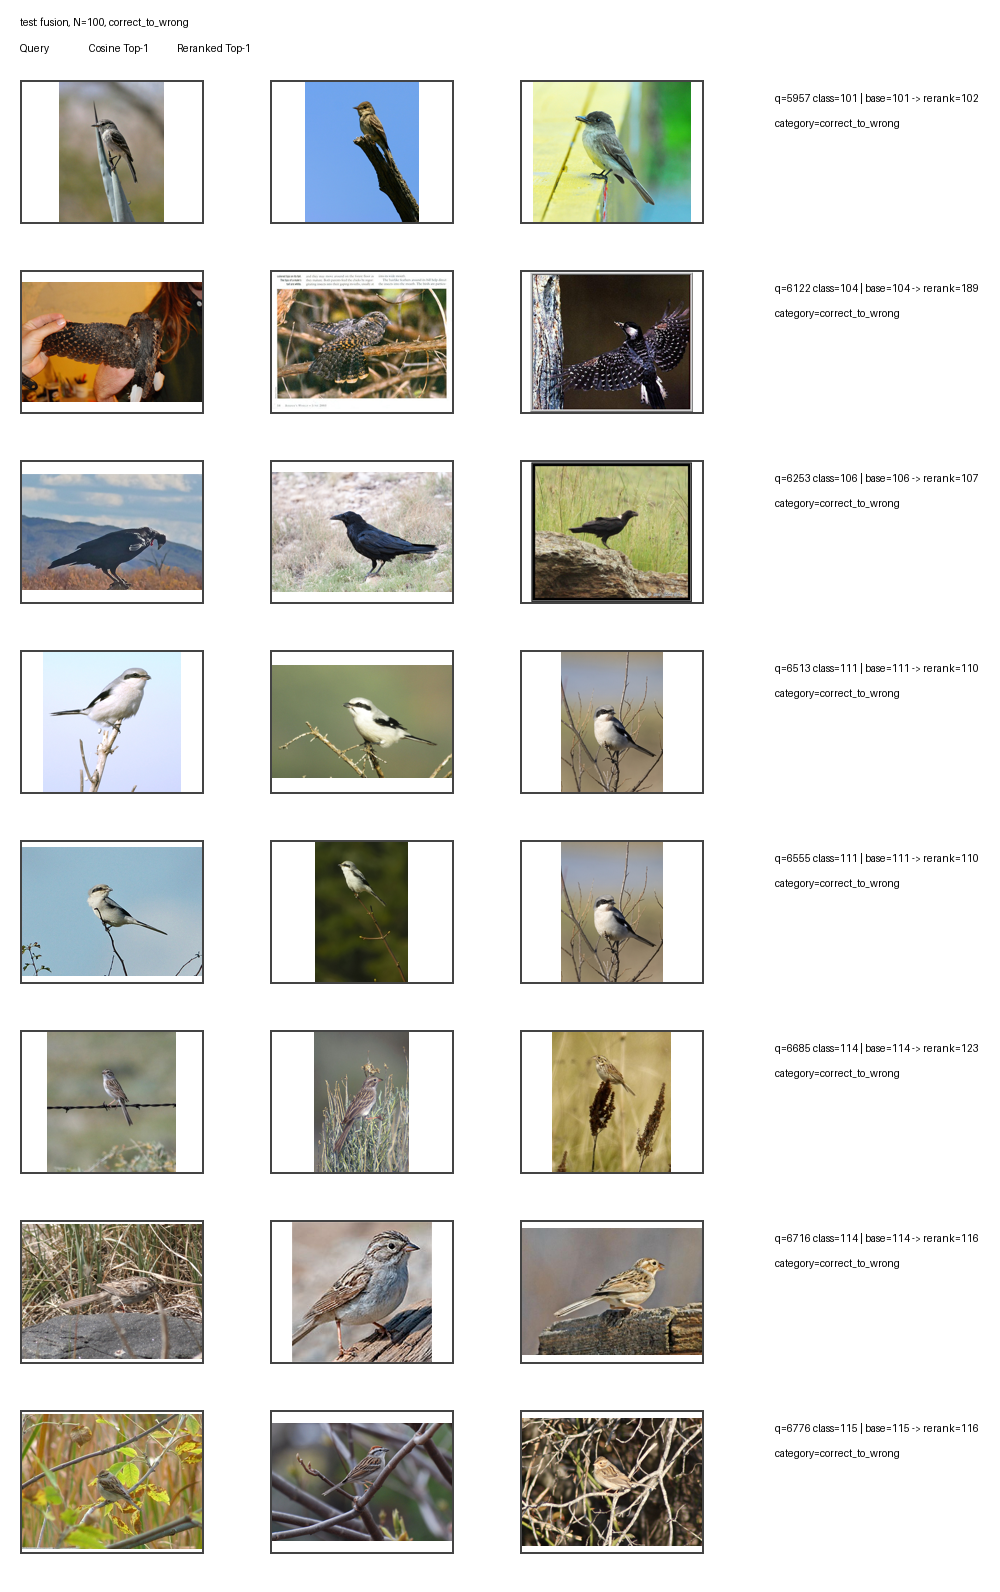
\includegraphics[width=0.92\textwidth]{fusion_correct_to_wrong.png}
\caption{Các trường hợp Fusion làm Top-1 đúng thành sai. Việc số trường hợp
sửa đúng và làm sai bằng nhau giải thích Recall@1 không thay đổi.}
\end{figure}

\section{Thảo luận}
Kết quả thống nhất giữa E1 và E2B: uncertainty của một ảnh không đo trực tiếp
khả năng ảnh đó phù hợp với một query cụ thể. Khi $N$ tăng, hard reranking theo
uncertainty phá vỡ ngày càng nhiều thứ tự cosine đúng. Pair-wise Confidence
khắc phục một phần vì nhìn đồng thời query và candidate, nhưng vẫn kém cosine
khi dùng riêng.

Fusion cho kết quả hợp lý hơn vì cosine tiếp tục là tín hiệu chính. Với
$\lambda=0{,}75$, confidence chỉ điều chỉnh các trường hợp gần nhau. Dù R@2,
R@4 và R@8 tăng nhẹ, bằng chứng hiện tại chưa cho thấy mức tăng ổn định. E2B
chỉ có một seed và test classes 100--199 đã được dùng trước đó để chọn
representation E2A; vì vậy kết quả test không phải một đánh giá hoàn toàn độc
lập và bootstrap chỉ mang ý nghĩa mô tả trên benchmark hiện tại.

Baseline E1 có 5.213 Hits@1, trong khi baseline E2B/E2A có 5.214 Hits@1. Đây
là hai feature cache được trích xuất ở hai pipeline riêng. Mọi so sánh trong
từng bảng vẫn dùng chung cache và ranking của chính thực nghiệm đó; không trộn
baseline E1 với kết quả E2B.

\section{Kết luận}
Image Uncertainty Reranking không cải thiện truy hồi DINOv3 và suy giảm nhanh
khi tăng Top-$N$. Pair-wise Confidence tốt hơn rõ rệt so với Image Uncertainty
trong điều kiện cùng tập train và cùng số ứng viên, nhưng chưa thể thay cosine.
Fusion với trọng số cosine lớn giữ nguyên R@1 và cải thiện rất nhỏ các Recall@K
còn lại. Hướng tiếp theo nên tập trung vào hiệu chỉnh confidence, nhiều seed
cho E2B và một benchmark độc lập chưa từng dùng để chọn phương pháp.

\section*{Tài liệu tham khảo}
\begin{enumerate}
  \item A. Simeoni et al., \emph{DINOv3}, 2025.
  \href{https://arxiv.org/abs/2508.10104}{arXiv:2508.10104}.
  \item M. Sensoy, L. Kaplan, M. Kandemir, \emph{Evidential Deep Learning to
  Quantify Classification Uncertainty}, 2018.
  \href{https://arxiv.org/abs/1806.01768v3}{arXiv:1806.01768v3}.
  \item D. Đorđević, S. Kumar, \emph{Evidential Transformers for Improved
  Image Retrieval}, 2025.
  \href{https://arxiv.org/abs/2409.01082v2}{arXiv:2409.01082v2}.
  \item C. Wah et al., \emph{The Caltech-UCSD Birds-200-2011 Dataset}, 2011.
\end{enumerate}

\end{document}
